\documentclass[12pt]{article}

\usepackage[margin=1in]{geometry}
\usepackage{amsmath,amsthm,amssymb}
\usepackage{mathrsfs}
\usepackage{mathtools}
\usepackage{enumitem}
\usepackage{physics}
\usepackage{pdfpages}

\newcommand{\magsq}[1]{\big|#1\big|^2}
\newcommand{\avg}[1]{\left<#1\right>}

\begin{document}
	
\title{Homework 4}
\author{Sean Ericson \\ Phys 684}
\maketitle

\section*{Problem 1}
\begin{enumerate}[label=(\alph*)]
    \item Letting
    \[ \vec{R} = \mqty(u\\v\\w); \quad \vec{\Omega} = \mqty(\Omega'_0\\-\Omega''_0\\\delta), \] 
    the evolution of the Bloch vector in the field interaction basis is given by
    \[
        \dv{t}\vec{R} = \vec{\Omega}\times\vec{R} \implies
        \begin{cases*}
            \dot{u} = -\delta v - \Omega_0'' w & \\
            \dot{v} = \delta u -\Omega_0' w & \\
            \dot{w} = \Omega_0' v + \Omega_0'' u. & \\
        \end{cases*} 
    \]
    Given that $\Omega_0' = \Omega_0$ and $\Omega_0'' = 0$ during the pulse, this simplifies to
    \begin{align*}
        \dot{u} &= -\delta v \\
        \dot{v} &= \delta u -\Omega_0 w \\
        \dot{w} &= \Omega_0 v.
    \end{align*}
    Then,
    \begin{alignat*}{3}
        &\quad & \ddot{v} &= \delta\dot{u} -\Omega_0\dot{w} \\
        &\quad & &= -\left(\delta^2 + \Omega_0^2\right)v \\
        &\quad & &= -\Omega^2v \\
        &\implies\quad & v(t) &= A\cos(\Omega t) + B\sin(\Omega t).
    \end{alignat*}
    Next, the initial condition $\vec{R}(0) = -\hat{w}$ implies $A = 0$, so
    \[ v(t) = B\sin(\Omega t). \]
    Now solving for u,
    \begin{alignat*}{3}
        &\quad & \dot{u} &= -\delta v \\
        &\implies\quad & u(t) &= u(0) - \delta\int_0^t\dd t' v(t') \\
        &\quad & &= \frac{\delta B}{\Omega}\cos(\Omega t')\big\vert_0^t \\
        &\quad & &= \frac{\delta B}{\Omega}\left(\cos(\Omega t) - 1\right),
    \end{alignat*}
    and then $w$
    \begin{alignat*}{3}
        &\quad & \dot{w} &= \Omega_0 v \\
        &\implies\quad & w(t) &= u(0) + \Omega_0\int_0^t\dd t' v(t') \\
        &\quad & &= -1 -\frac{\Omega_0 B}{\Omega}\cos(\Omega t')\big\vert_0^t \\
        &\quad & &= -1 -\frac{\Omega_0 B}{\Omega}\left(\cos(\Omega t) - 1\right)
    \end{alignat*}
    Using the equation for $\dot{v}$ we can determine the value of $B$:
    \begin{alignat*}{3}
        &\quad & \dot{v} &= \delta u - \Omega_0 w \\
        &\implies\quad & \Omega B \cos(\Omega t) & = \frac{\delta^2B}{\Omega}\left(\cos(\Omega t) - 1\right) + \Omega_0\left(1 + \frac{\Omega_0B}{\Omega}\left(\cos(\Omega t) - 1\right)\right) \\
        &\quad & &= \frac{\delta^2 + \Omega_0^2}{\Omega}B\cos(\Omega t) - \frac{\delta^2 + \Omega_0^2}{\Omega}B + \Omega_0 \\
        &\quad & &= \Omega B\cos(\Omega t) - \Omega B  + \Omega_0 \\
        &\implies\quad & \Omega B &= \Omega_0 \\
        &\implies\quad & B &= \frac{\Omega_0}{\Omega}.
    \end{alignat*}
    After the pulse ends the precession of the Bloch vector stops, and its final position is given by $\vec{R}(\tau)$. Letting $\theta = \Omega\tau$,
    \begin{align*}
        u &= \frac{\Omega_0\delta}{\Omega^2}\left(\cos\theta - 1\right) \\
        v &= \frac{\Omega_0}{\Omega}\sin\theta \\
        w &= -\left[1 + \frac{\Omega_0^2}{\Omega^2}\left(\cos\theta - 1\right)\right].
    \end{align*}
\end{enumerate}

\section*{Problem 2}
See attached Mathematica notebook.

\section*{Problem 3}
See attached Mathematica notebook.

\section*{Problem 4}
See attached Mathematica notebook for calculations.
\[ H_\text{d} = -\frac{\hbar}{2}\Omega_0\sigma_z + \hbar\dot{\theta}\sigma_y \]
\begin{align*}
    \dot{\tilde{\rho}}_\text{d} &= \comm{H_\text{d}}{\tilde{\rho}_\text{d}} \\
    &= \mqty(-\dot{\theta}\Re[\tilde{\rho_d}_{12}] & i\Omega_0\rho_{12}-\dot{\theta}\left(\tilde{\rho_d}_{22} - \tilde{\rho_d}_{11}\right) \\ -i\Omega_0\rho_{21}-\dot{\theta}\left(\tilde{\rho_d}_{22} - \tilde{\rho_d}_{11}\right) & \dot{\theta}\Re[\tilde{\rho_d}_{12}])
\end{align*}

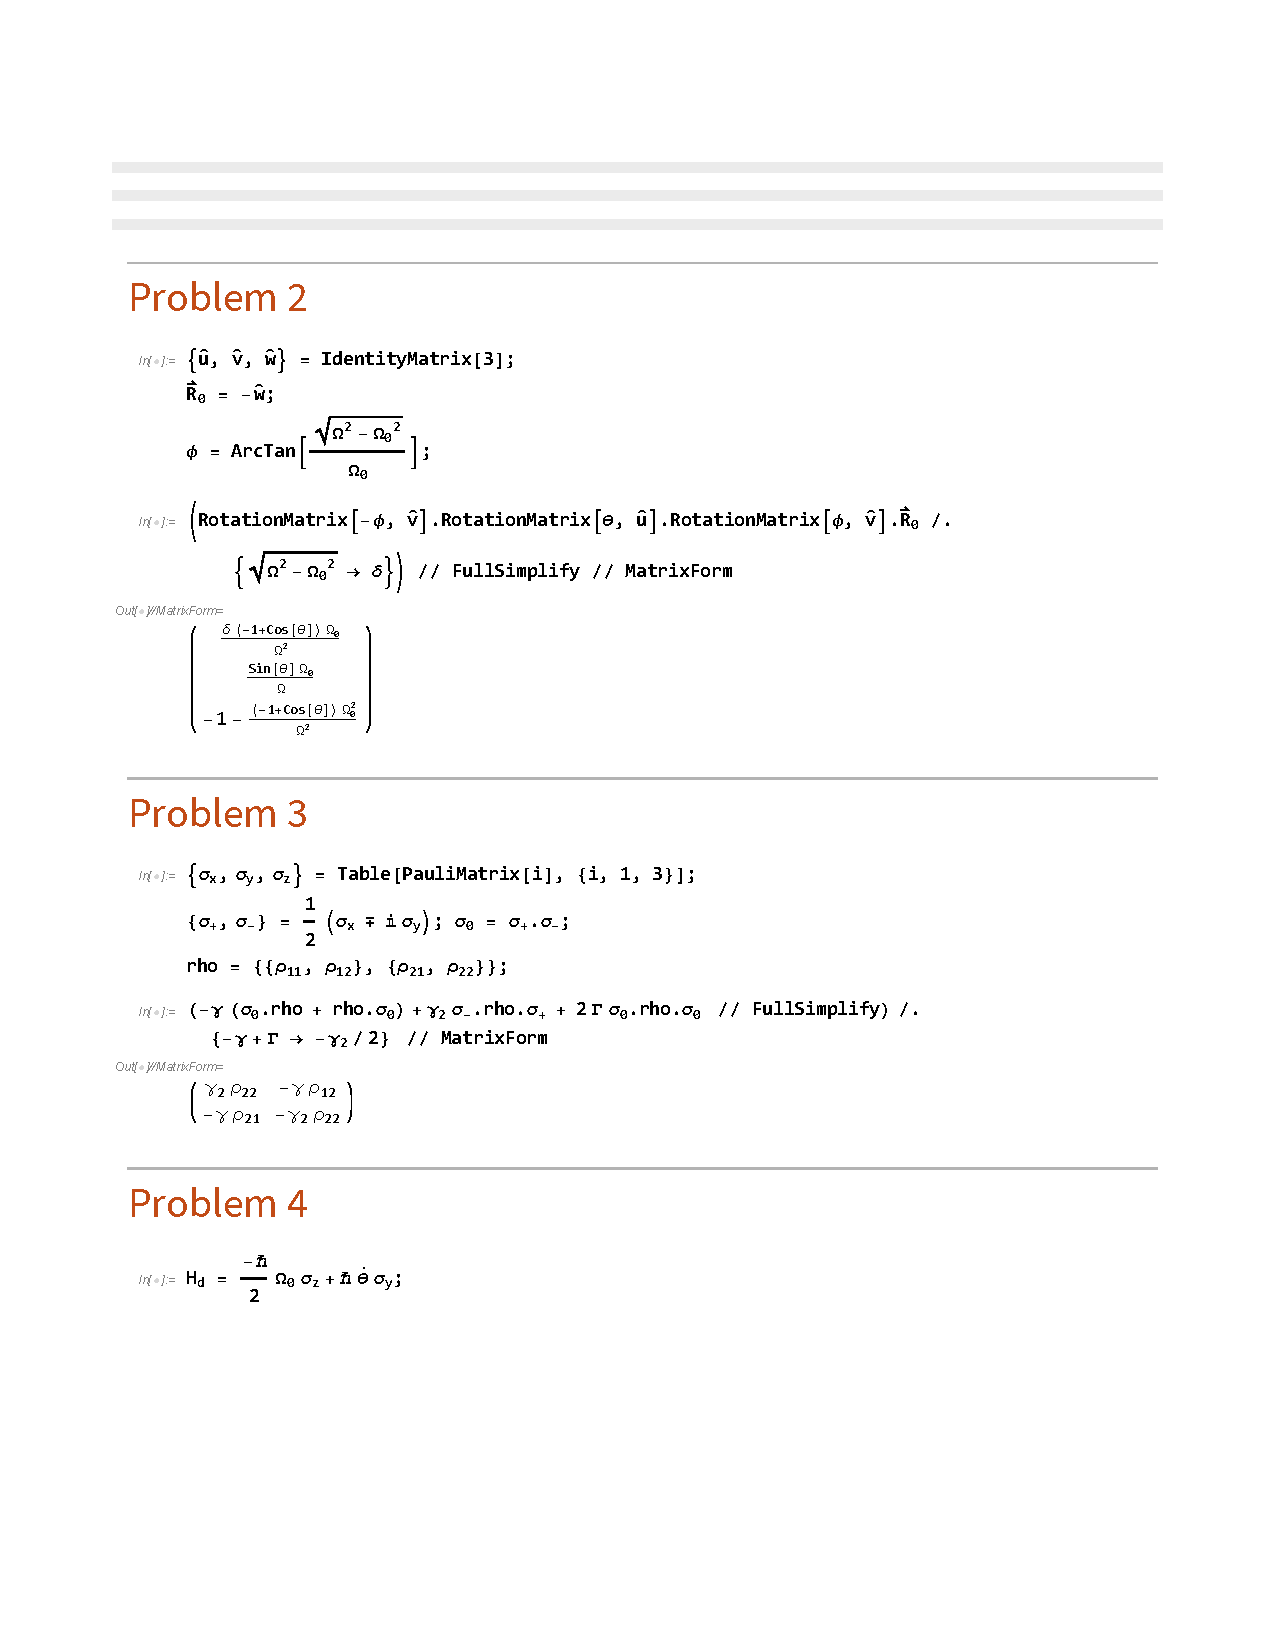
\includepdf[pages=-]{calcs/HW4_mathematica.pdf}
\end{document}